\documentclass[a4paper,11pt]{article}

\usepackage[utf8]{inputenc} \usepackage[T1]{fontenc}
\usepackage{fancyhdr} \usepackage{graphicx,subfig} \usepackage{lastpage}
\usepackage{amssymb,amsmath} \usepackage{siunitx} \usepackage[nodayofweek]{datetime}
\usepackage[top=3.5cm,bottom=2.5cm,left=3cm,right=3cm,headheight=40pt]{geometry}
\usepackage{parskip} \usepackage{float} \usepackage{enumitem} \pagestyle{fancy}
\usepackage[colorlinks=true,allcolors=blue]{hyperref} \hypersetup{
	pdfauthor={Michaël Defferrard},
	pdftitle={Project stage 3: Interaction \& Animation},
	pdfsubject={Introduction to Computer Graphics}
}

\lhead{Introduction to Computer Graphics\\Project stage 3: Interaction \& Animation\\Group 19}
\chead{\hspace{2.5cm}EPFL\\\hspace{2.5cm}\shortdate\today\\\hspace{2.5cm}\thepage/\pageref{LastPage}}
\rhead{Michaël \textsc{Defferrard}\\Pierre \textsc{Fechting}\\Vu Hiep \textsc{Doan}}
\cfoot{}

\begin{document}


\section{Overview}

This report presents our advancement on the third part of the project : interaction and animation. During all the run of the project, we focused on code architecture and quality rather than quantity. It would have been impossible to implement every single idea we had about the project anyway.
%At this stage, we realized that we are better technicians than artists.

We did implement all the basic

\section{Implementation}

\subsection{Basic - Fly through mode}

In order to freely fly through our scene, the camera mode free fly provide 3 possible actions:
\begin{itemize}
\item go forward/backward.
\item turn left/right.
\item turn up/down.
\end{itemize}
To have all possible rotation, the camera has to rotate on virtual axis, see figure \ref{freefly_rotation} present the behavior of a user turning up and then right creating a virtual axis of rotation.
\begin{figure}[ht]
	\centering
	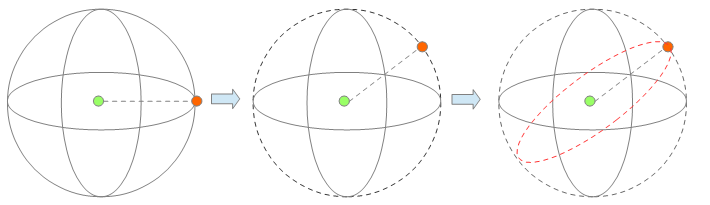
\includegraphics[height=4cm]{{{img_stage3/cameraFreeFly}}}
 	\caption{Free flying rotation example}
 	\label{freefly_rotation}
\end{figure}
To achieve such rotations,the look at point has to be displaced staying always at equal distance to the camera position. We proceed this rotation in 3 steps: 
translate to origin, undo previous rotations, do new rotations, return to initial placement. Rotations are proceeded only in two axis, Y and Z, using rotation matrix computed according to inputs angle. A velocity has been added, the acceleration is gradual until a maximum value, same behavior for deceleration. 

\subsection{Basic - FPS exploration mode}

The FPS exploration mode has slightly different rotation behavior. Camera's rotations are expected to reproduce similar effect as the head rotation of a human body. In this purpose the lateral rotations will always be proceeded on a virtual axis parallel to the world horizontal axis. An example of such behavior is represented figure \ref{fps_rotation}.  
\begin{figure}[ht]
	\centering
	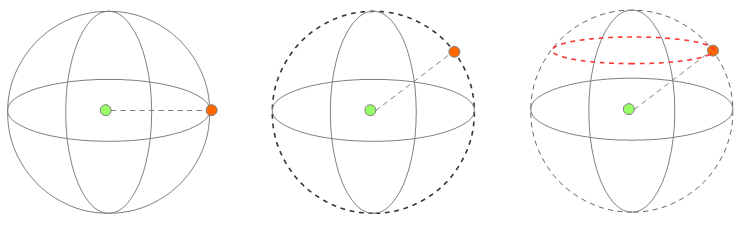
\includegraphics[height=4cm]{{{img_stage3/cameraFPS}}}
 	\caption{Fps rotation example}
 	\label{fps_rotation}
\end{figure}
Thus, transformation is simplified for lateral rotations compared to free flying mode. Vertical rotation stays similar.
In order to have a smooth walk in our scene, the Z component of the camera position is equal to the mean of the 24 positions around camera x-y position, avoiding camera shaking in sharp terrain.

\subsection{Advanced - Physically realistic movements}

In order to have movement physically more realistic, an acceleration/deceleration has been added to every movement, body will not instantaneously move. An additional running function has been added to increase a maximum forward speed higher.
A simple jump function has been created, it uses a sinus to shape the jump z variations. Jumping speed vary according to the jump stage, beginning/ending of the jump has a higher speed then higher steps.In the case of jumping from the top of a mountain, the falling speed will reach a maximum value and keep falling at constant speed until it reach the floor.
While jumping the trajectory is computed using the action settled just before the jump. For example, if a user was turning, the rotation will continue during jump making a spinning effect, which will decelerate once the users reach the floor again. 

\subsection{Advanced - Camera path control}


\subsection{Advanced - Pictorial camera}


\subsection{Advanced - Water modeling}

Water refraction, reflection and depth

For the water reflection effect, we should render the terrain from a flipped camera position. The terrain is thus rendered two times. It is rendered a first time with the real camera position to the default framebuffer (screen) and a second time with a flipped virtual camera position to a texture which is attached to a framebuffer object. The texture is later used to render the water surface.

\subsection{Advanced - Particle system}

The cheapest way to display particles is to use sprites: polygons that face the camera
in any orientation.

As for the heightmap, if we were able to work with OpenGL 4, we could have use compute shaders instead of an empty vertex shader for this kind of GPGPU computation. It would have permit us to store particle data in buffer objects and avoid pingpong storage.

%Each sprite is created using the Geometry Shader. So we only feed the GPU a set of 3D positions, one per sprite. The Geometry Shader expands each position into two triangles and correctly orients them perpendicular to the camera view direction.
transparency gradient proportional to distance to center : \texttt{gl\_PointCoord}
particle size inversely proportional to the squared distance to the camera : \texttt{gl\_pointSize}
no sorting with respect to camera distance for transparency : can create weird effect if a particle that is nearer than another gets drawn before. The farther particle will visually seem to be in front of the nearer. Thanks to particle speed, this won't be visible.
Draw a real flocon ? not much added value to particle speed
Use geometry shader ?
Particle texture ?
A common technique to solve this is to test if the currently-drawn fragment is near the Z-Buffer. If so, the fragment is faded out. However, you’ll have to sample the Z-Buffer, which is not possible with the “normal” Z-Buffer. You need to render your scene in a render target. Alternatively, you can copy the Z-Buffer from one framebuffer to another with glBlitFramebuffer.

As we cannot read from a texture and render to it at the same time, we need two velocity textures. The one used as an input is the one that was rendered to before. At each frame rendering we exchange the two.

The vertex attribute buffer contain integers from 0 to nParticles - 1. The attribute is the index in the \texttt{particlesPosTex} which will allow the \texttt{particles\_render\_vshader} to retrieve the particle position. The attribute type is \texttt{GL\_INT}. As for the indices to not be converted to floating point values, the \texttt{glVertexAttribIPointer} function is used (notice the \texttt{I}).

The \texttt{gl\_VertexID} vertex language input variable is used by the \texttt{particule\_render\_vshader} to index the particle textures.
1D texture to store position and velocity.
Window and textures are of size \texttt{nParticles} times 1 pixels.

In our implementation, particles that fall below the water level are reseted to the top and will fall down again, indefinitely. In order to keep the aggregate compact and so as it does not spread out in the space, particles that go too far in x or y direction get moved to the oder side.

discard is used

\subsection{Advanced - Two simultaneous views}

By two simultaneous views, we mean the rendering of the seen from two points of views. In our case, a control view and a camera view (fig.). The control view is used to set the camera path Bézier curve control points and have a global view with an animated pictorial camera. The camera view actually shows what the camera sees.

The keyboad ENTER key can be used to exchange the two views (fig.).

From an implementation point of view, almost each object of the scene (skybox, terrain, water, shadowmap, skybox, particles) should be drawn from two different points of view. They are thus rendered to two FBOs (with attached output texture and depth buffer) instead of the default framebuffer (the screen). The \texttt{Display} class eventually uses the texture to assemble the final screen view.

For performance reason, it is crucial to render the two points of view one after the other as shader program switch is expensive.


\section{Improvements on last stage}

\subsection{Code cleanup}

As this hand-in is the last opportunity to modify our code, we put great effort in improving its quality by cleaning it up, including comments. A great job was done to functionalize shader code. As a side effect, we did also discover some little mistakes. We did also refactor most of the code to encompass our new object oriented architecture introduced in stage 2. In overall, code quality has greatly improved.

Redeclare the GLSL built-in blocks : \texttt{gl\_PerVertex} to be able to use separable program objects.\footnote{\url{http://www.geeks3d.com/20130106/nvidia-updates-its-opengl-sdk/}}

Use \texttt{glProgramUniform} instead of \texttt{glUniform}. The former takes a program ID argument which indicates in which program it should retrieve the uniform ID. Using this function it is no more needed to have the program marked as used by \texttt{glUseProgram}.

By testing our code on Window and Linux with a combination of ATI and Nvidia hardware and drivers, we found quite some interesting corner-cases where the OpenGL specification is not entirely met. An example is the size of the \texttt{gl\_ClipDistance} array of the \texttt{gl\_PerVertex} block. According to the spec\footnote{\url{https://www.opengl.org/sdk/docs/man4/html/gl\_ClipDistance.xhtml}}, the

\subsection{Vertices object}

To achieve better modulation, we have separated the vertices creation code into a class hierarchy. The \texttt{Vertices} base class is an abstract class, declaring only virtual methods, which defines the interface. The \texttt{VerticesQuad}, \texttt{VerticesGrid} and \texttt{VerticesSkybox} inherit from it and implement the \texttt{generate} \texttt{draw} and \texttt{clean} methods which are specific to them. This design allows more than one \text{RenderingContext} object to share a \texttt{Vertices} object. The \texttt{Terrain} and \texttt{Shadowmap} makes use of this. It also offers better source code modularity.

\subsection{Lightning}

Phong shading was improperly implemented at stage 2. The material texture was only used to compute the ambient color. The diffuse and specular colors were fixed for all the terrain. Probably a reminiscent of stage 1. This is now fixed. We first retrieve material color properties from textures. The retrieved color is then split across the three lightnings (ambient, diffuse and specular) with the help of coefficients which some up to 1. The specular lightning coefficient is non-zero for water only. The water uses two normals : a normalmap for diffuse lightning (this is used to create the impression of water movement) and a (0,0,1) normal for specular lightning (this is used to create the impression of sun light reflection).

The light direction was defined in stage 2 to be the same for all the vertices. This defines it as a directional light. It was changed to a spot light (or point light in the lightning context), to be coherent with shadowing. The shadowmap is indeed computed using perspective projection, not orthographic.

\subsection{Shadowmap}

We have improved a lot the shadowmap, as it was not yet working properly at Stage 2. Figure~\ref{shadowmap} shows how it works by showing the shadowmap, the distance to light and the rendered terrain for three different light positions. While we were at shadowmap, we also took the time to test some parameters.

\begin{figure}[ht]
	\centering
	\subfloat[Shadowmap at position 2]{
		\label{shadowmap_depth_2}
		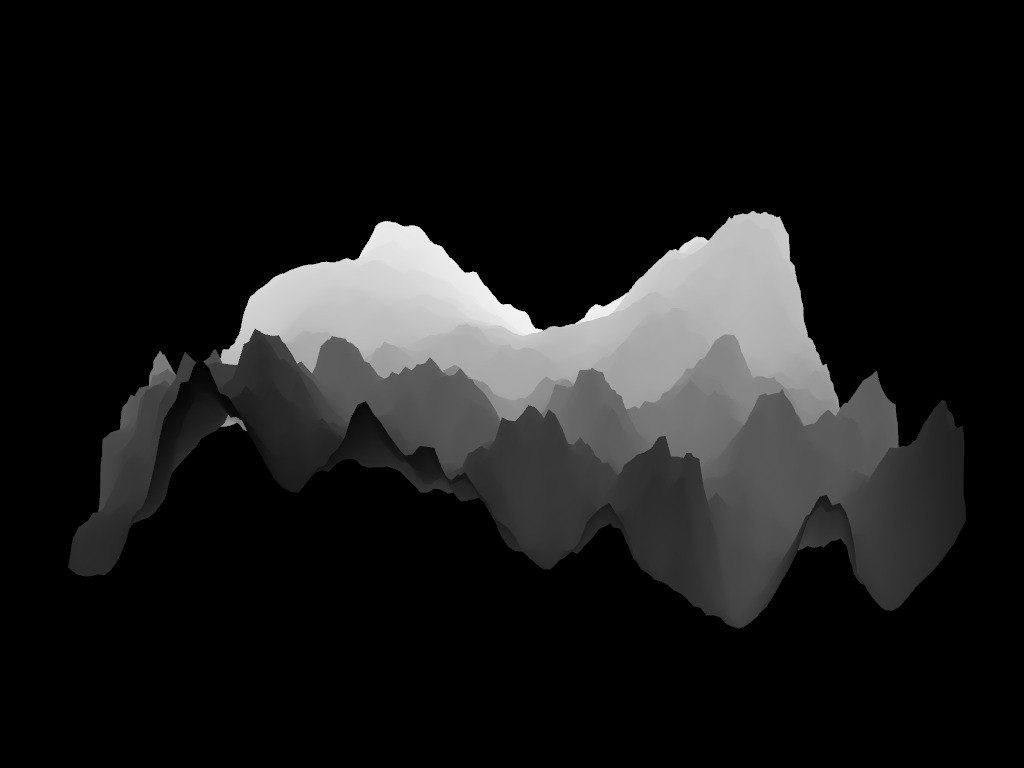
\includegraphics[height=3cm]{{{img_stage3/shadowmap_depth_2}}}
	} \quad
	\subfloat[Shadowmap at position 5]{
		\label{shadowmap_depth_5}
		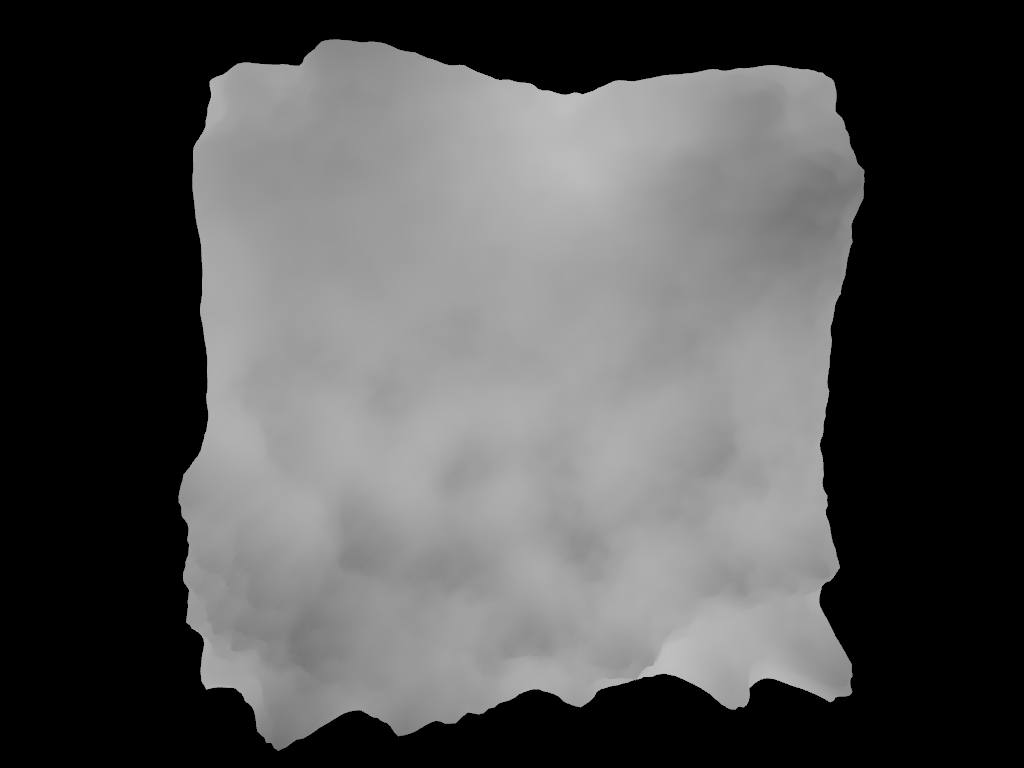
\includegraphics[height=3cm]{{{img_stage3/shadowmap_depth_5}}}
	} \quad
	\subfloat[Shadowmap at position 7]{
		\label{shadowmap_depth_7}
		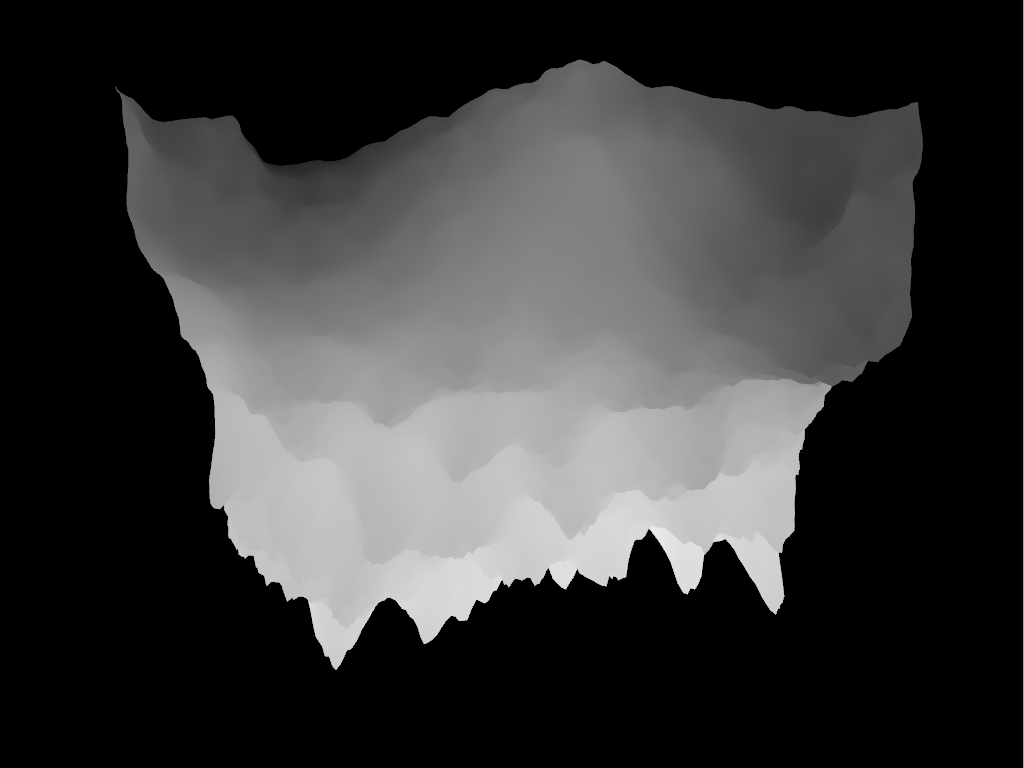
\includegraphics[height=3cm]{{{img_stage3/shadowmap_depth_7}}}
	} \\
	\subfloat[Distance at position 2]{
		\label{shadowmap_distance_2}
		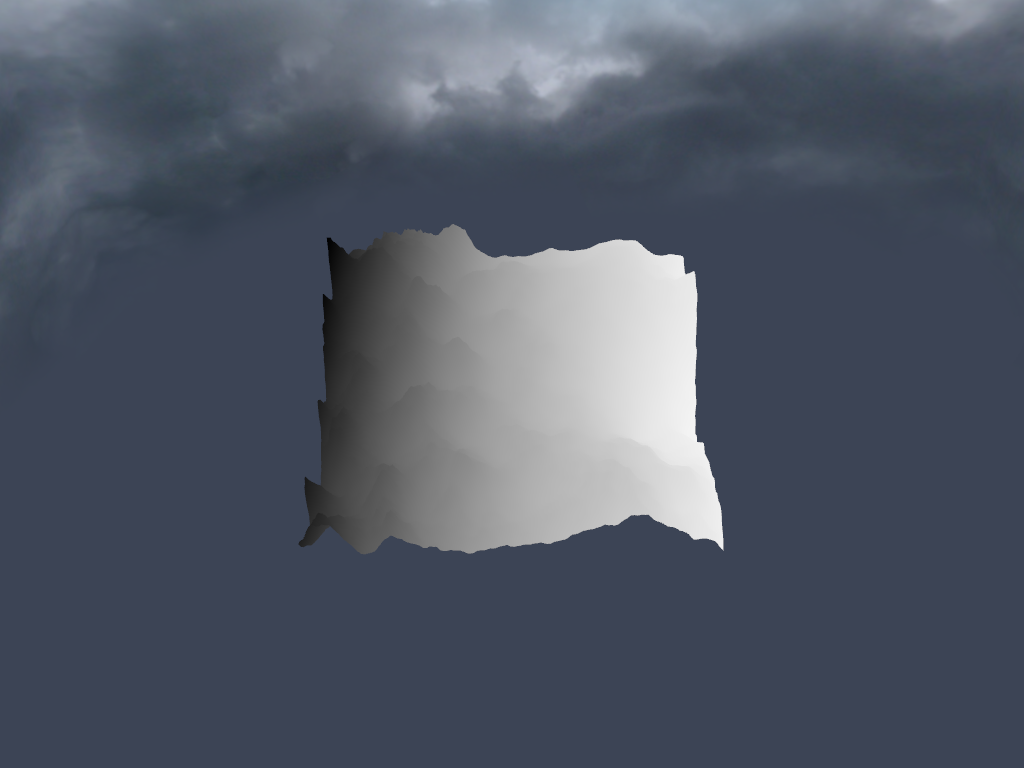
\includegraphics[height=3cm]{{{img_stage3/shadowmap_distance_2}}}
	} \quad
	\subfloat[Distance at position 5]{
		\label{shadowmap_distance_5}
		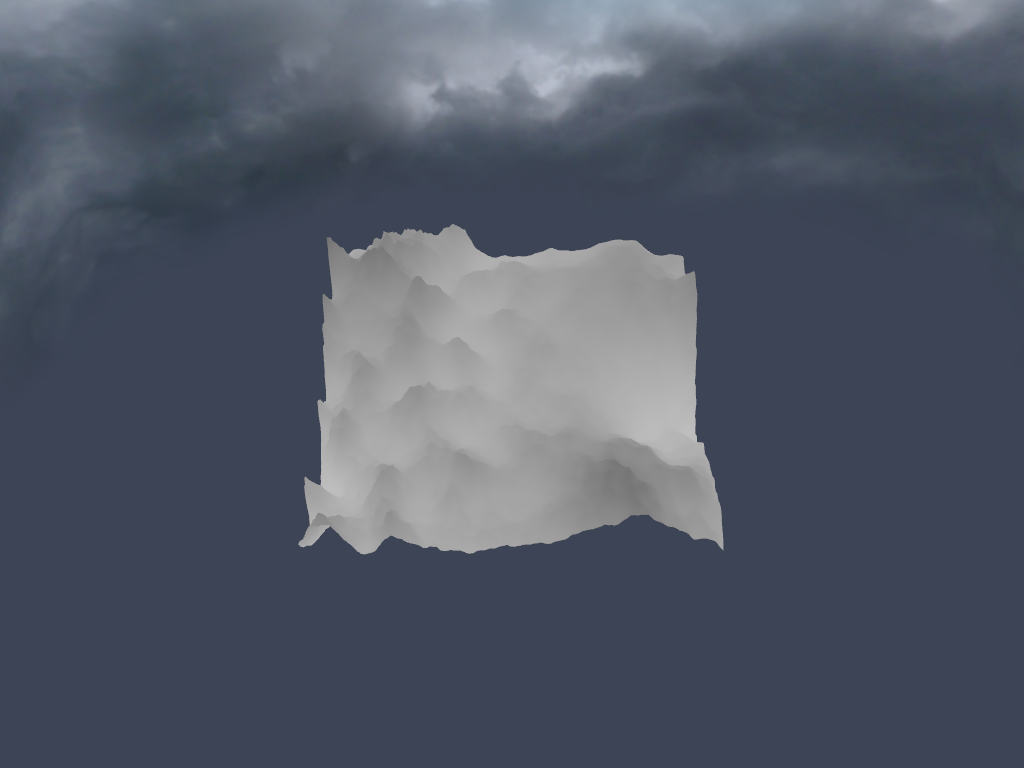
\includegraphics[height=3cm]{{{img_stage3/shadowmap_distance_5}}}
	} \quad
	\subfloat[Distance at position 7]{
		\label{shadowmap_distance_7}
		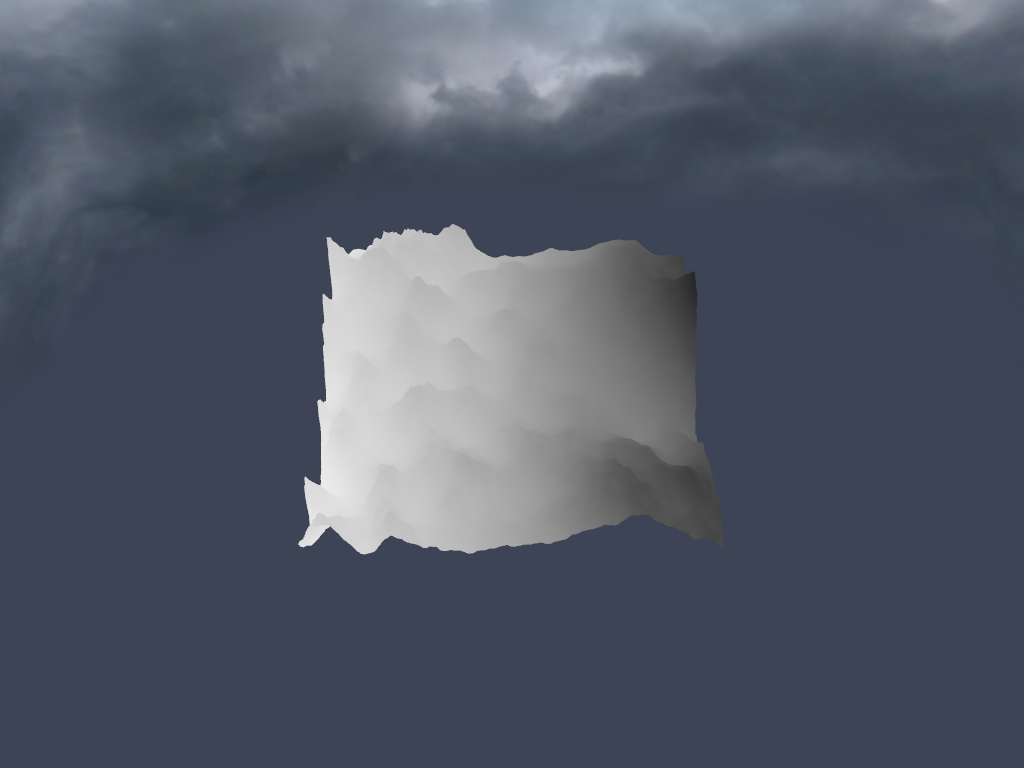
\includegraphics[height=3cm]{{{img_stage3/shadowmap_distance_7}}}
	} \\
	\subfloat[Terrain at position 2]{
		\label{shadowmap_terrain_2}
		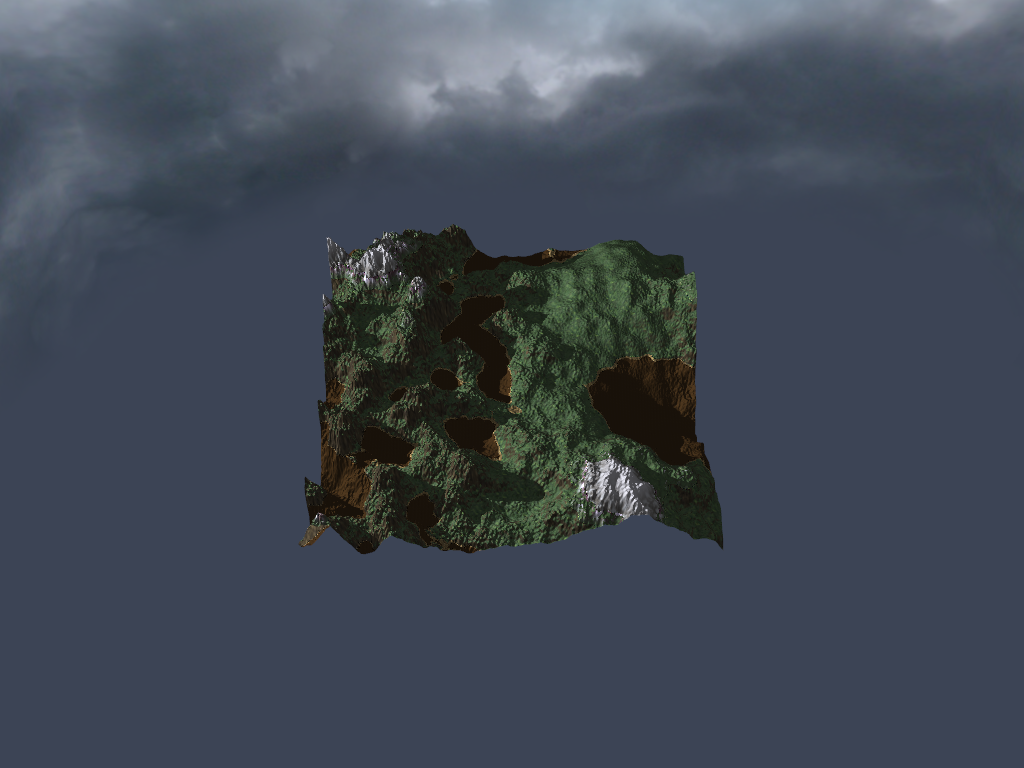
\includegraphics[height=3cm]{{{img_stage3/shadowmap_terrain_2}}}
	} \quad
	\subfloat[Terrain at position 5]{
		\label{shadowmap_terrain_5}
		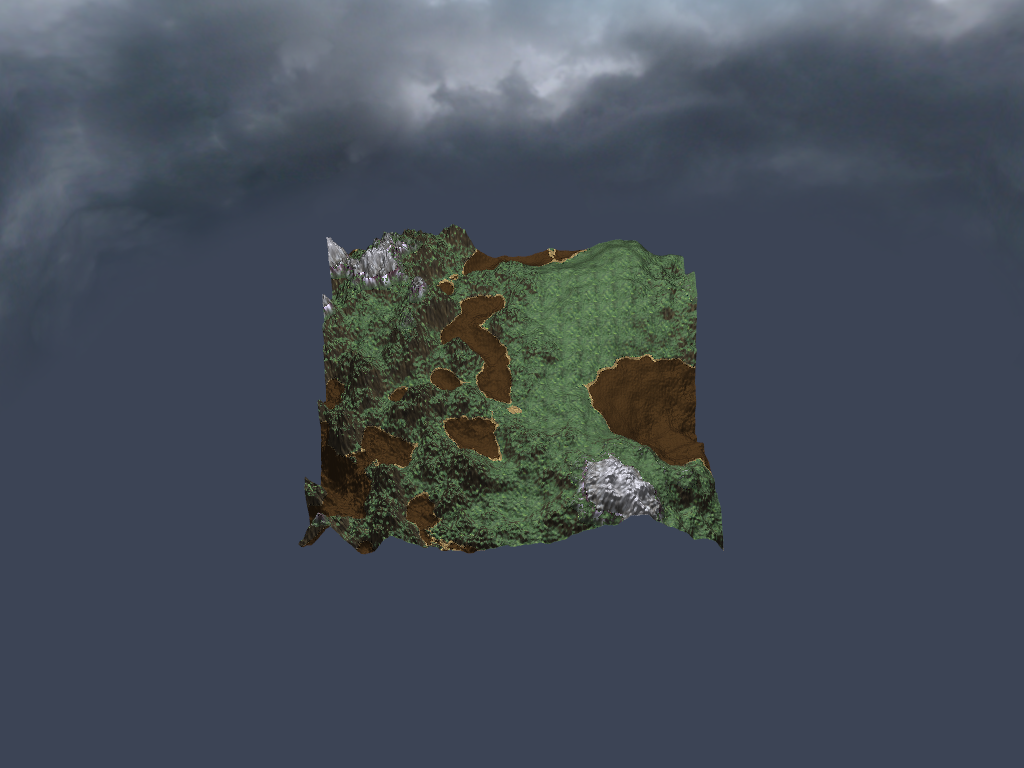
\includegraphics[height=3cm]{{{img_stage3/shadowmap_terrain_5}}}
	} \quad
	\subfloat[Terrain at position 7]{
		\label{shadowmap_terrain_7}
		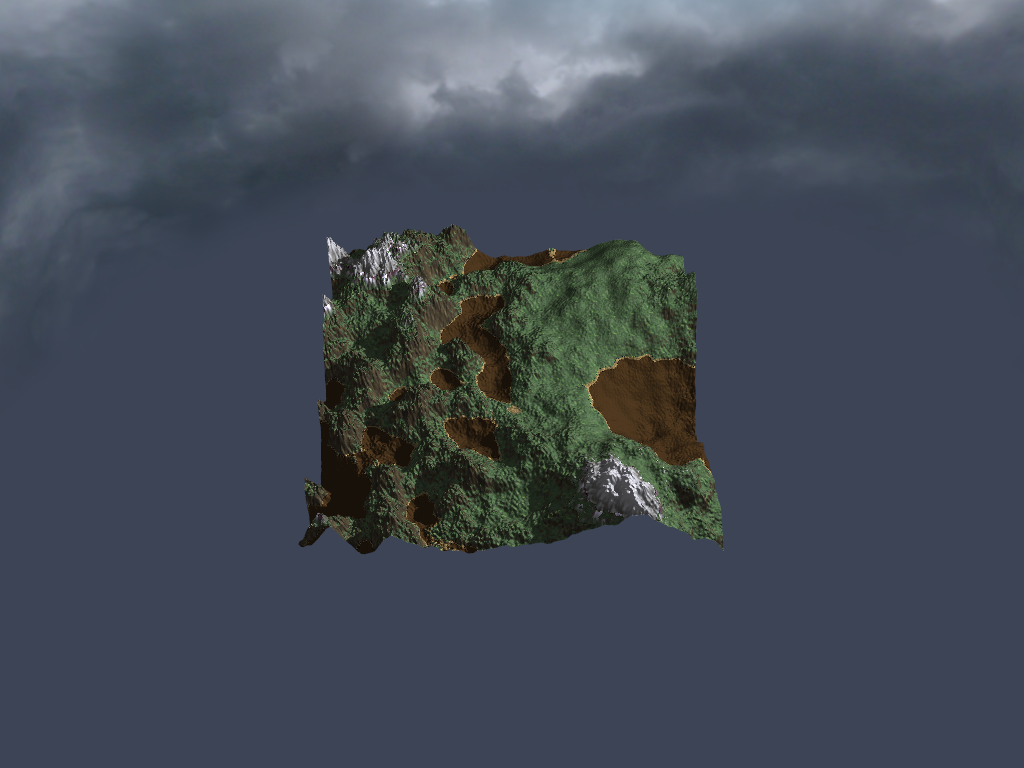
\includegraphics[height=3cm]{{{img_stage3/shadowmap_terrain_7}}}
	}
	\caption{Shadowmap construction}
	\label{shadowmap}
\end{figure}

The division by the w component to apply projection should be done before the coordinates change from (-1,-1)x(1,1) to (0,0)x(1,1). It can thus not be integrated in the \texttt{lightMVP} matrix and should be computed by the shader. To save computations and GPU memory bandwidth (passing a \texttt{vec3} instead of a \texttt{vec4}), this can also be computed by the vertex shader. The result is then interpolated and passed to the fragment shader. The differences are very small, as shown by figures~\ref{shadowmap_coord_fshader} and~\ref{shadowmap_coord_vshader}.

\begin{figure}[ht]
	\centering
	\subfloat[In fragment shader]{
		\label{shadowmap_coord_fshader}
		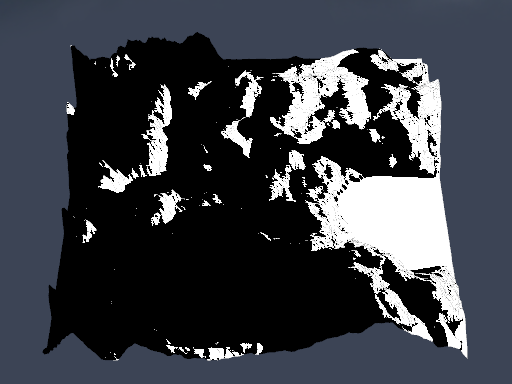
\includegraphics[height=4cm]{{{img_stage3/shadowmap_coord_fshader}}}
	} \quad
	\subfloat[In vertex shader]{
		\label{shadowmap_coord_vshader}
		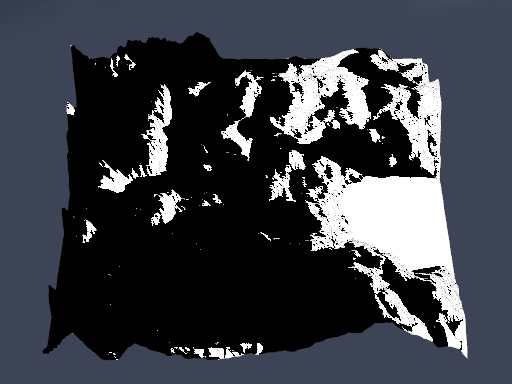
\includegraphics[height=4cm]{{{img_stage3/shadowmap_coord_vshader}}}
	}
	\caption{Coordinates transform}
	\label{shadowmap_coord}
\end{figure}

The choice of the bias, used when comparing the distance to light with the one stored in the shadowmap has an impact. A too low value will result in Z-buffer fighting (fig.~\ref{shadowmap_bias_no}) while a too big value will result in shadow errors (fig.~\ref{shadowmap_bias_big}). A good compromise should be found (fig.~\ref{shadowmap_bias_ok}).

\begin{figure}[ht]
	\centering
	\subfloat[No bias]{
		\label{shadowmap_bias_no}
		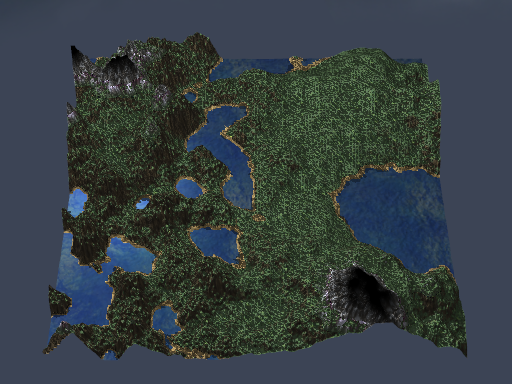
\includegraphics[height=3cm]{{{img_stage3/shadowmap_bias_no}}}
	} \quad
	\subfloat[Good value]{
		\label{shadowmap_bias_ok}
		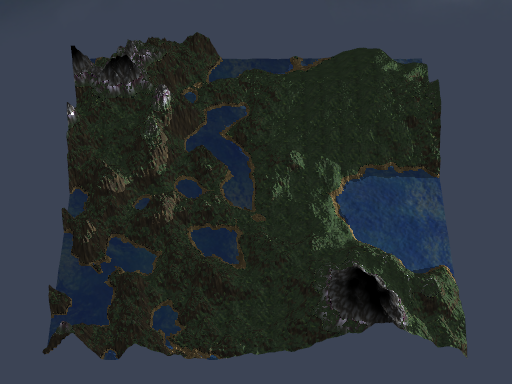
\includegraphics[height=3cm]{{{img_stage3/shadowmap_bias_ok}}}
	} \quad
	\subfloat[Too big value]{
		\label{shadowmap_bias_big}
		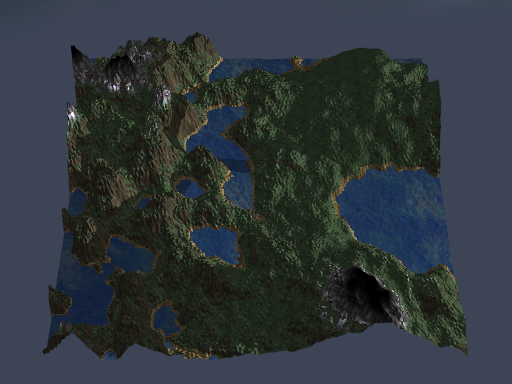
\includegraphics[height=3cm]{{{img_stage3/shadowmap_bias_big}}}
	}
	\caption{Shadowmap with different bias values}
	\label{shadowmap_bias}
\end{figure}

Percentage closer filtering (PCF), a method which sample four neighboring pixels and return an average of the tests, greatly smooth the transition between shadow and light regions. Figures~\ref{shadowmap_32bits_PCFwith} and~\ref{shadowmap_32bits_PCFwithout} show the same scene with and without PCF. The effect on transitions is clear.

\begin{figure}[ht]
	\centering
	\subfloat[32 bits depth without PCF]{
		\label{shadowmap_32bits_PCFwithout}
		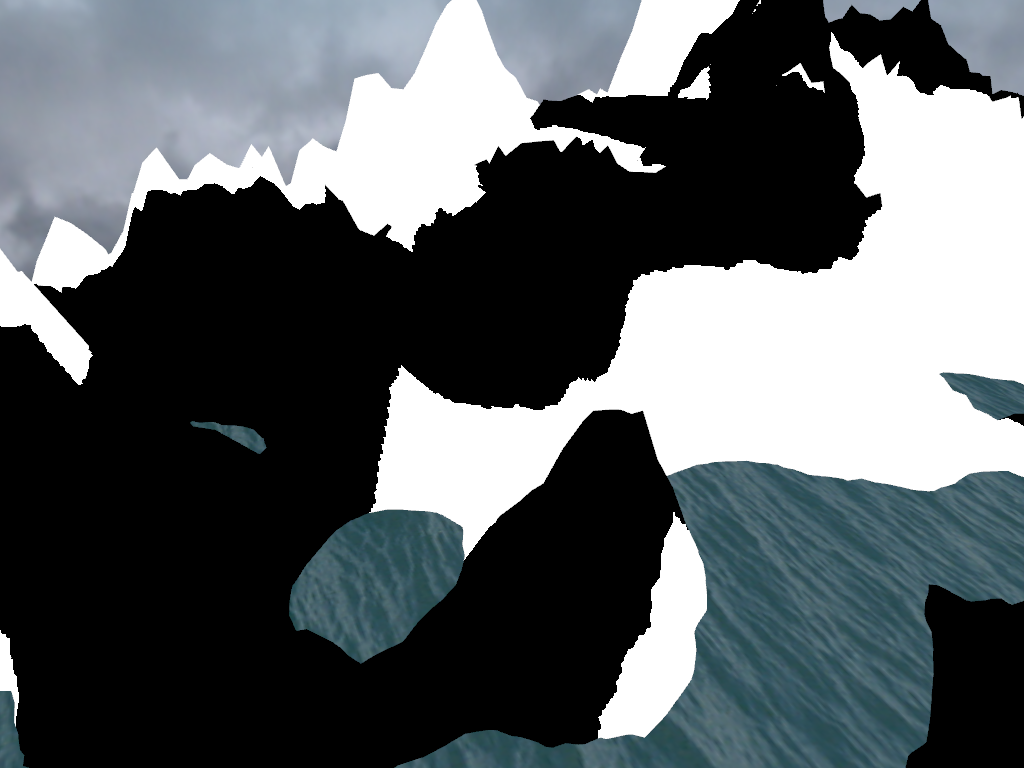
\includegraphics[height=3cm]{{{img_stage3/shadowmap_32bits_PCFwithout}}}
	} \quad
	\subfloat[32 bits depth with PCF]{
		\label{shadowmap_32bits_PCFwith}
		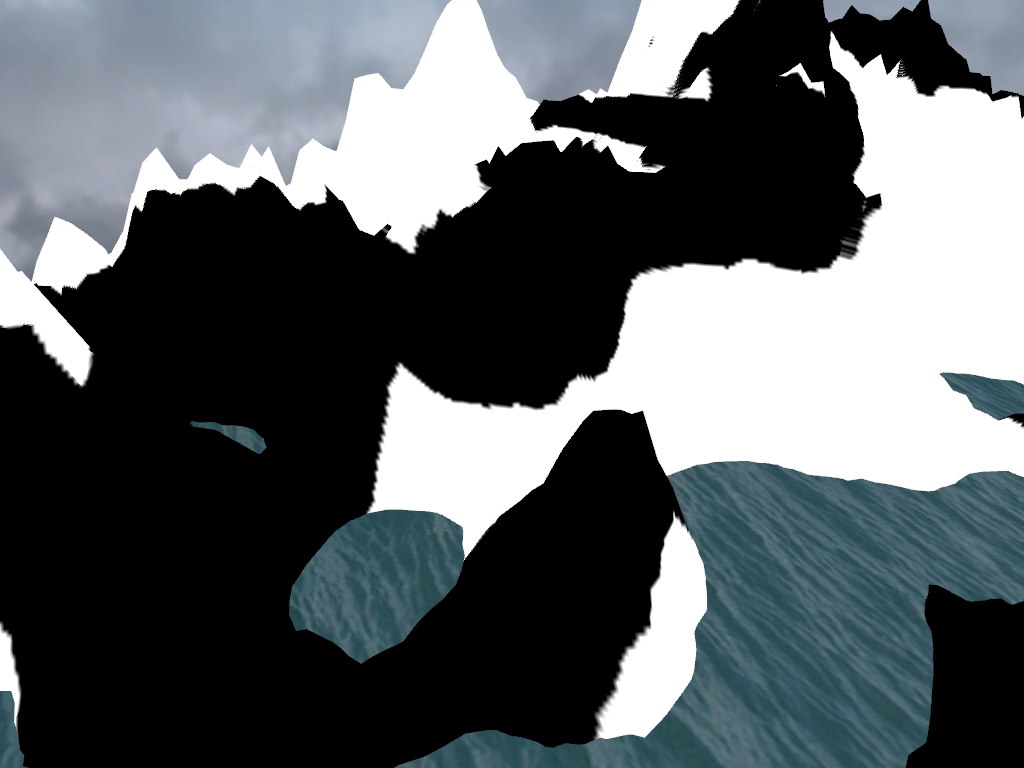
\includegraphics[height=3cm]{{{img_stage3/shadowmap_32bits_PCFwith}}}
	} \quad
	\subfloat[16 bits depth with PCF]{
		\label{shadowmap_16bits_PCFwith}
		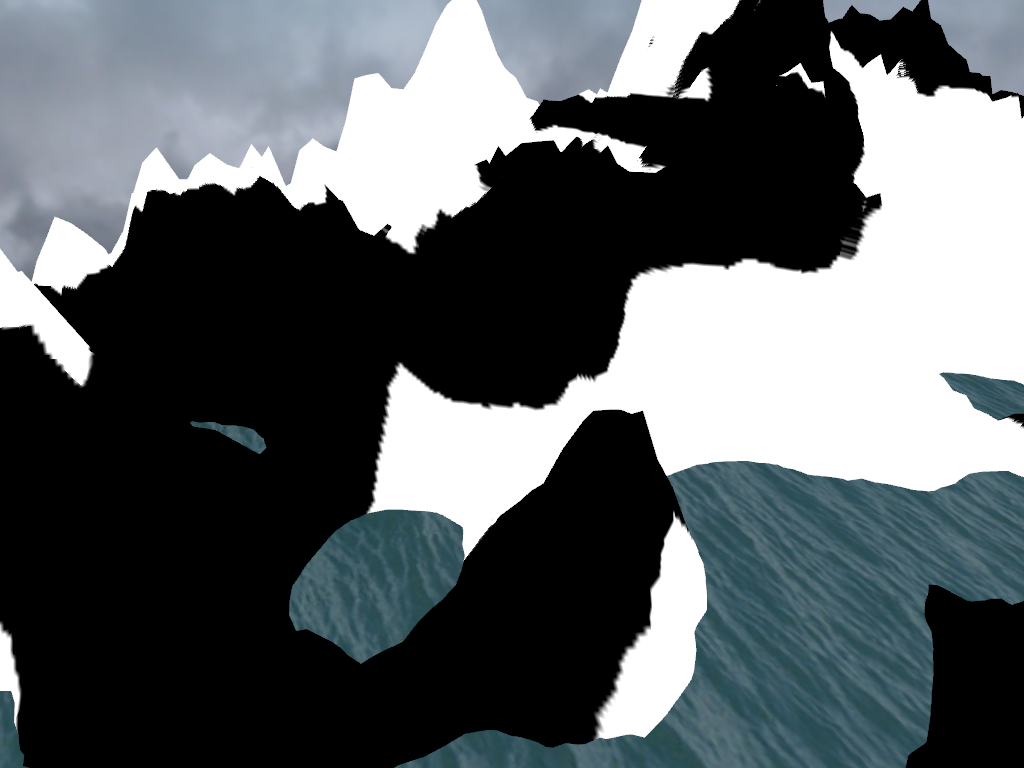
\includegraphics[height=3cm]{{{img_stage3/shadowmap_16bits_PCFwith}}}
	}
	\caption{Shadowmap}
	\label{shadowmap_bits_PCF}
\end{figure}

The differences between a 32 bits depth buffer (fig.~\ref{shadowmap_32bits_PCFwith}) or a 16 bits (fig.~\ref{shadowmap_16bits_PCFwith}) depth buffer is very little. We have thus chosen 16 bits to save computation time and memory space.

\subsection{Heightmap}

The heightmap texture was configured with the default heuristic for out-of-range values. This default is to wrap around the texture (\texttt{GL\_REPEAT}) which creates artifacts at the borders of the terrain (fig.~\ref{heightmap_artifacts}). Clamping the texture coordinates (\texttt{GL\_CLAMP\_TO\_EDGE}) to the [0,1] range eliminates the artifacts (fig.~\ref{heightmap_ok}).

\begin{figure}[ht]
	\centering
	\subfloat[With artifacts at the border]{
		\label{heightmap_artifacts}
		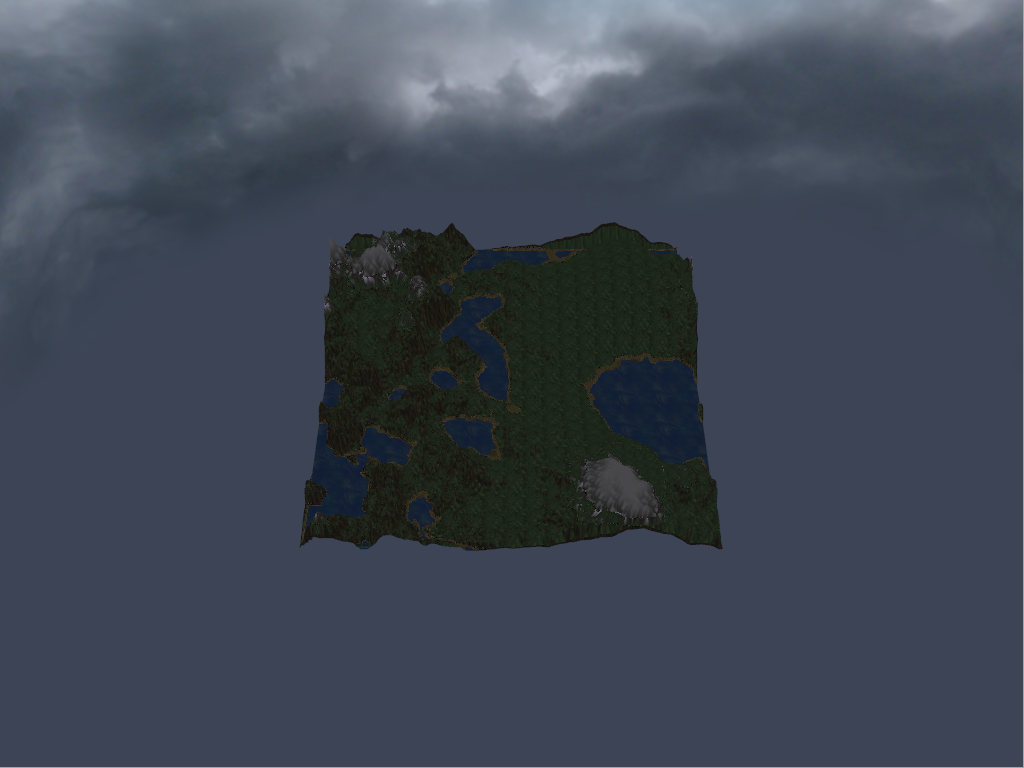
\includegraphics[height=4cm]{{{img_stage3/heightmap_artifacts}}}
	} \quad
	\subfloat[Without artifacts]{
		\label{heightmap_ok}
		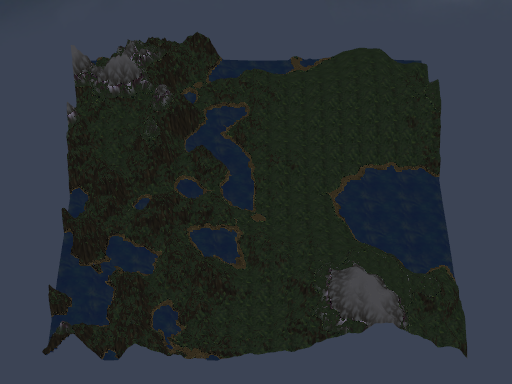
\includegraphics[height=4cm]{{{img_stage3/heightmap_ok}}}
	}
	\caption{Heightmap}
	\label{heightmap}
\end{figure}

The heightmap code was also refactored to accommodate our new object oriented architecture. This resulted in a cleaner design and better readability as well as some improvements of the generic code.

Another improvement of the heightmap code is that the \texttt{position} vector is now a \texttt{vec2} instead of a \texttt{vec3} as the vertex z position of a quad is 0 anyway. This saves some GPU memory bandwidth.

\section{Results}


\end{document}
